\section{Group Actions}

\subsection{Group Actions and Permutation Representations}

Let $G$ be a group and let $A$ be a nonempty set.

\begin{problems}
    \item Let $G$ act on the set $A$. Prove that if $a,b \in A$ and $b = g \cdot a$ for some $g \in G$, then \(G_b = g G_a g^{-1}\) (\(G_a\) is the stabilizer of $a$). Deduce that if $G$ acts transitively on $A$ then the kernel of the action is
    \[\bigcap_{g \in G} g G_a g^{-1}.\]
    \begin{sol}
		Suppose $h \in G_b$. We want to show that $h \in gG_ag\inv$. Since $h \in G_b$, we have $h \cdot b = b$. But $b = g \cdot a$, so $h \cdot (g \cdot a) = g \cdot a$. Applying $g\inv$ to both sides, we get $g\inv h g \cdot a = a$. This means that $g\inv h g \in G_a$, so $h \in g G_a g\inv$. Thus, we have shown that \(G_b \subseteq g G_a g^{-1}\). For the other direction, suppose $h \in g G_a g^{-1}$. Then there exists some $k \in G_a$ such that $h = g k g^{-1}$. We want to show that $h \in G_b$. We have $h \cdot b = (g k g^{-1}) \cdot (g \cdot a) = g \cdot (k \cdot a) = g \cdot a = b$, since $k \in G_a$ implies $k \cdot a = a$. Thus, $h \in G_b$. Therefore, we have shown that \(g G_a g^{-1} \subseteq G_b\). Combining both inclusions, we conclude that \(G_b = g G_a g^{-1}\).

		Now, if $G$ acts transitively on $A$, then for any $b \in A$, there exists some $g \in G$ such that $b = g \cdot a$. From the first part, we have \(G_b = g G_a g^{-1}\). The kernel of the action is the intersection of all stabilizers \(G_b\) for \(b \in A\). Therefore, the kernel is
		\[\bigcap_{b \in A} G_b = \bigcap_{g \in G} g G_a g^{-1}. \qh\]
	\end{sol}
    \item Let $G$ be a permutation group on the set $A$ (i.e., \(G \leq S_A\)), let \(\sigma \in G\) and let \(a \in A\). Prove that \(\sigma G_a \sigma^{-1} = G_{\sigma(a)}\). Deduce that if $G$ acts transitively on $A$ then 
    \[\bigcap_{\sigma \in G} \sigma G_a \sigma^{-1} = 1.\]
    \begin{sol}
		Suppose $\tau \in \sigma G_a\sigma\inv$. We want to show that $\tau \in G_{\sigma(a)}$. Since $\tau \in \sigma G_a \sigma^{-1}$, there exists some $\rho \in G_a$ such that $\tau = \sigma \rho \sigma^{-1}$. We have $\tau \cdot \sigma(a) = (\sigma \rho \sigma^{-1}) \cdot \sigma(a) = \sigma \cdot (\rho \cdot a) = \sigma(a)$, since $\rho \in G_a$ implies $\rho \cdot a = a$. Thus, $\tau \in G_{\sigma(a)}$. Therefore, we have shown that \(\sigma G_a \sigma^{-1} \subseteq G_{\sigma(a)}\). For the other direction, suppose $\tau \in G_{\sigma(a)}$. We want to show that $\tau \in \sigma G_a \sigma^{-1}$. We have $\tau \cdot \sigma(a) = \sigma(a)$. Applying $\sigma^{-1}$ to both sides, we get $\sigma^{-1} \tau \sigma \cdot a = a$. This means that $\sigma^{-1} \tau \sigma \in G_a$, so $\tau \in \sigma G_a \sigma^{-1}$. Thus, we have shown that \(G_{\sigma(a)} \subseteq \sigma G_a \sigma^{-1}\). Combining both inclusions, we conclude that \(\sigma G_a \sigma^{-1} = G_{\sigma(a)}\).

		Now, if $G$ acts transitively on $A$, then for any $b \in A$, there exists some $\sigma \in G$ such that $b = \sigma(a)$. From the first part, we have \(\sigma G_a \sigma^{-1} = G_b\). The kernel of the action is the intersection of all stabilizers \(G_b\) for \(b \in A\). Therefore, the kernel is
		\[\bigcap_{b \in A} G_b = \bigcap_{\sigma \in G} \sigma G_a \sigma^{-1} = 1. \qh\]
	\end{sol}
    \item Assume that $G$ is an abelian, transitive subgroup of $S_A$. Show that \(\sigma(a) \neq a\) for all \(\sigma \in G - \{1\}\) and all \(a \in A\). Deduce that \(|G| = |A|\). [Use the preceding exercise.]
    \begin{sol}
		Since $G$ is abelian, then the conjugate of $G_a$ is trivial, i.e., $\sigma G_a \sigma\inv = G_a$ for all $\sigma \in G$. From the previous exercise, we know that the kernel of this action is trivial. However, the intersection of all $\sigma G_a\sigma\inv$ is just $G_a$ so that $G_a = 1$. Then $G_a$ is trivial for every $a \in A$, hence $\sigma(a) \neq a$ for all $\sigma \in G - \{1\}$ and all $a \in A$. It follows by Proposition 4.2 that $|G|/|G_a| = |A|$, hence $|G| = |A|$ because $G_a$ is trivial.
	\end{sol}
    \item Let \(S_3\) act on the set \(\Omega\) of ordered pairs \(\{(i,j) \mid 1 \le i,j \le 3\}\) by \(\sigma((i,j)) = (\sigma(i), \sigma(j))\). Find the orbits of \(S_3\) on \(\Omega\). For each \(\sigma \in S_3\) find the cycle decomposition of \(\sigma\) under this action (i.e., find its cycle decomposition when \(\sigma\) is considered as an element of \(S_9\)—first fix a labeling of these nine ordered pairs). For each orbit \(\mathcal{O}\) of $S_3$ acting on these nine points, pick some \(a \in \mathcal{O}\) and find the stabilizer of \(a\) in \(S_3\).
    \begin{sol}
		Note that in $\Omega$, there are two types of ordered pairs: those with identical elements and those with distinct elements. In the former case, it is clear that any $\sigma \in S_3$ will map such a pair to another pair with identical elements. In the latter case, it is easy to find some $\sigma \in S_3$ that maps any ordered pair with distinct elements to any other such pair. We now label the elements of $\Omega$ accordingly:
		\begin{multicols}{3}
			\begin{itemize}
				\item 1 = (1, 1)
				\item 2 = (2, 2)
				\item 3 = (3, 3)
				\item 4 = (1, 2)
				\item 5 = (2, 1)
				\item 6 = (1, 3)
				\item 7 = (3, 1)
				\item 8 = (2, 3)
				\item 9 = (3, 2)
			\end{itemize}
		\end{multicols}
		We then have the two orbits 
		\[\oo_1 = \{(i, i) \mid i \in \set{1, 2, 3}\} \longand \oo_2 = \set{(i, j) \mid i \neq j}\]
		of $S_3$ acting on $\Omega$. Note that $|\oo_1| = 3$ and $|\oo_2| = 6$. Now for each $\sigma \in S_3$, we find its cycle decomposition as an element of $S_9$. We describe how to compute one such cycle decomposition, and the rest follow similarly. Consider $\sigma = (1 2 3) \in S_3$. Then we have the following mappings:
		\begin{itemize}
			\item $(1, 1) \mapsto (2, 2) \mapsto (3, 3) \mapsto (1, 1)$, which corresponds to the cycle $(1\ 2\ 3)$ in $S_9$.
			\item $(1, 2) \mapsto (2, 3) \mapsto (3, 1) \mapsto (1, 2)$, which corresponds to the cycle $(4\ 8\ 7)$ in $S_9$.
			\item $(2, 1) \mapsto (3, 2) \mapsto (1, 3) \mapsto (2, 1)$, which corresponds to the cycle $(5\ 9\ 6)$ in $S_9$.
		\end{itemize}
		Combining these cycles, we find that the cycle decomposition of $\sigma = (1 2 3)$ in $S_9$ is $(1\ 2\ 3)(4\ 8\ 7)(5\ 9\ 6)$. The cycle decompositions for all elements of $S_3$ acting on $\Omega$ are as follows:
		\begin{multicols}{3}
			\begin{itemize}
				\item $1 \in S_3$ is the same as $1 \in S_9$.
				\item $(1 2)$: $(1\ 2)(4\ 5)(6\ 7)(8\ 9)$
				\item $(1 3)$: $(1\ 3)(4\ 6)(5\ 7)(8\ 9)$
				\item $(2 3)$: $(1\ 2)(2\ 3)(5\ 6)(7\ 8)$
				\item $(1 2 3)$: $(1\ 2\ 3)(4\ 8\ 7)(5\ 9\ 6)$
				\item $(1 3 2)$: $(1\ 3\ 2)(4\ 7\ 8)(5\ 6\ 9)$
			\end{itemize}
		\end{multicols}
		For $\oo_1$, we pick $a = (1, 1)$. The only $\sigma \in S_3$ that fixes $(1, 1)$ is the identity permutation and $(2\ 3)$, so the stabilizer of $(1, 1)$ in $S_3$ is $\gen{(2\ 3)}$. Moreover, we have $|G_a||\oo_1| = 2 \cdot 3 = 6 = |S_3|$ as expected. For $\oo_2$, we pick $a = (1, 2)$. The only $\sigma \in S_3$ that fixes $(1, 2)$ is the identity permutation, so the stabilizer of $(1, 2)$ in $S_3$ is 1. Again, $|G_a||\oo_2| = 1 \cdot 6 = 6 = |S_3|$.
	\end{sol}
    \item For each of parts (a) and (b) repeat the preceding exercise but with $S_3$ acting on the specified set:
    \begin{problems}
        \item the set of 27 triples \(\{(i,j,k) \mid 1 \le i,j,k \le 3\}\)
        \item the set \(\mathcal{P}(\{1,2,3\}) - \{\emptyset\}\) of all 7 nonempty subsets of \(\{1,2,3\}\)
    \end{problems}
    \begin{solalph}
		\item We begin by classifying these set of triples. There are five types of triples:
		\begin{itemize}
			\item Type 1: Triples with all identical elements.
			\item Type 2: Triples whose two first coordinates are identical.
			\item Type 3: Triples whose first and last coordinates are identical.
			\item Type 4: Triples whose last two coordinates are identical.
			\item Type 5: Triples with all distinct elements.
		\end{itemize}
		Note that this is a correct classification. One may suggest to combine Types 2, 3, and 4 into a singular type. However, observe that no elements may be permuted such that the location of a pair of identical coordinates move to another one, i.e., there is no such permutation $\sigma$ in $S_3$ such that $(1, 1, 2)$ maps to $(1, 2, 2)$.We now label the elements of $\Omega$ lexicographically as follows, i.e., we begin by increasing the last coordinate, then increasing the middle coordinate, and finally increasing the first coordinate:
		\begin{multicols}{3}
			\begin{itemize}
				\item $1 = (1, 1, 1)$
				\item $2 = (1, 1, 2)$
				\item $3 = (1, 1, 3)$
				\item $4 = (1, 2, 1)$
				\item $5 = (1, 2, 2)$
				\item $6 = (1, 2, 3)$
				\item $7 = (1, 3, 1)$
				\item $8 = (1, 3, 2)$
				\item $9 = (1, 3, 3)$
				\item $10 = (2, 1, 1)$
				\item $11 = (2, 1, 2)$
				\item $12 = (2, 1, 3)$
				\item $13 = (2, 2, 1)$
				\item $14 = (2, 2, 2)$
				\item $15 = (2, 2, 3)$
				\item $16 = (2, 3, 1)$
				\item $17 = (2, 3, 2)$
				\item $18 = (2, 3, 3)$
				\item $19 = (3, 1, 1)$
				\item $20 = (3, 1, 2)$
				\item $21 = (3, 1, 3)$
				\item $22 = (3, 2, 1)$
				\item $23 = (3, 2, 2)$
				\item $24 = (3, 2, 3)$
				\item $25 = (3, 3, 1)$
				\item $26 = (3, 3, 2)$
				\item $27 = (3, 3, 3)$
			\end{itemize}
		\end{multicols}
		The classification yields the following orbits of $S_3$ acting on $\Omega$:
		\begin{itemize}
			\item $\oo_1 = \{(i, i, i) \mid i \in \set{1, 2, 3}\}$ with order 3.
			\item $\oo_2 = \{(i, i, j) \mid i \neq j\}$ with order 6.
			\item $\oo_3 = \{(i, j, i) \mid i \neq j\}$ with order 6.
			\item $\oo_4 = \{(j, i, i) \mid i \neq j\}$	with order 6.
			\item $\oo_5 = \{(i, j, k) \mid i, j, k \text{ distinct}\}$ with order 6.
		\end{itemize}
		The cycle decompositions for all elements of $S_3$ acting on $\Omega$ are as follows:
		\begin{itemize}
			\item $1 \in S_3$ is the same as $1 \in S_{27}$.
			\item $(1\ 2)$: $(1\ 14)(2\ 13)(3\ 15)(4\ 11)(5\ 10)(6\ 12)(7\ 17)(8\ 16)(9\ 18)(19\ 23)(20\ 22)(21\ 24)(25\ 26)$
			\item $(1\ 3)$: $(1\ 27)(2\ 26)(3\ 25)(4\ 24)(5\ 23)(6\ 22)(7\ 21)(8\ 20)(9\ 19)(10\ 18)(11\ 17)(12\ 16)(13\ 15)$
			\item $(2\ 3)$: $(2\ 3)(4\ 7)(5\ 9)(6\ 8)(10\ 19)(11\ 21)(12\ 20)(13\ 25)(14\ 27)(15\ 26)(16\ 22)(17\ 24)(18\ 23)$
			\item $(1\ 2\ 3)$: $(1\ 14\ 27)(2\ 15\ 25)(3\ 13\ 26)(4\ 17\ 21)(5\ 18\ 19)(6\ 16\ 20)(7\ 11\ 24)(8\ 12\ 22)(9\ 10\ 23)$
			\item $(1\ 3\ 2)$: $(1\ 27\ 14)(2\ 25\ 15)(3\ 26\ 13)(4\ 21\ 17)(5\ 19\ 18)(6\ 20\ 16)(7\ 24\ 11)(8\ 22\ 12)(9\ 23\ 10)$
		\end{itemize}
		For $\oo_1$, pick $a = (1\ 1\ 1)$. The elements that stabilize $a$ are the identity permutation and $(2\ 3)$, so the stabilizer of $a$ in $S_3$ is $\gen{(2\ 3)}$. We have $|G_a||\oo_1| = 2 \cdot 3 = 6 = |S_3|$. For the other orbits, note that $S_3$ acts transitively on each of them, so the stabilizer of any chosen element in these orbits is trivial. For example, for $\oo_2$, pick $a = (1\ 1\ 2)$. The only element that stabilizes $a$ is the identity permutation, so the stabilizer of $a$ in $S_3$ is 1. We have $|G_a||\oo_2| = 1 \cdot 6 = 6 = |S_3|$. The same logic applies to $\oo_3$, $\oo_4$, and $\oo_5$.
		\item We begin by classifying the nonempty subsets of $\{1, 2, 3\}$. There are three types of subsets: 1-element subsets, 2-element subsets, and the 3-element subset. We now label the elements of $\mathcal{P}(\{1, 2, 3\}) - \{\emptyset\}$ as follows:
		\begin{multicols}{4}
			\begin{itemize}
				\item $1 = \{1\}$
				\item $2 = \{2\}$
				\item $3 = \{3\}$
				\item $4 = \{1, 2\}$
				\item $5 = \{1, 3\}$
				\item $6 = \{2, 3\}$
				\item $7 = \{1, 2, 3\}$
			\end{itemize}
		\end{multicols}
		The classification yields the following orbits of $S_3$ acting on $\mathcal{P}(\{1, 2, 3\}) - \{\emptyset\}$:
		\begin{itemize}
			\item $\oo_1 = \{\{1\}, \{2\}, \{3\}\}$ with order 3.
			\item $\oo_2 = \{\{1, 2\}, \{1, 3\}, \{2, 3\}\}$ with order 3.
			\item $\oo_3 = \{\{1, 2, 3\}\}$ with order 1.
		\end{itemize}
		The cycle decompositions for all elements of $S_3$ acting on $\mathcal{P}(\{1, 2, 3\}) - \{\emptyset\}$ are as follows:
		\begin{itemize}
			\item $1 \in S_3$ is the same as $1 \in S_7$.
			\item $(1\ 2)$: $(1\ 2)(5\ 6)$
			\item $(1\ 3)$: $(1\ 3)(4\ 6)$
			\item $(2\ 3)$: $(2\ 3)(4\ 5)$
			\item $(1\ 2\ 3)$: $(1\ 2\ 3)(4\ 6\ 5)$
			\item $(1\ 3\ 2)$: $(1\ 3\ 2)(4\ 5\ 6)$
		\end{itemize}
		For $\oo_1$, pick $a = \{1\}$. The only elements that stabilize $a$ are the identity permutation and $(2\ 3)$, so the stabilizer of $a$ in $S_3$ is $\gen{(2\ 3)}$. We have $|G_a||\oo_1| = 2 \cdot 3 = 6 = |S_3|$. For $\oo_2$, pick $a = \{1, 2\}$. The only elements that stabilize $a$ are the identity permutation and $(1\ 2)$, so the stabilizer of $a$ in $S_3$ is $\gen{(1\ 2)}$. We have $|G_a||\oo_2| = 2 \cdot 3 = 6 = |S_3|$. For $\oo_3$, note that $S_3$ acts trivially on this orbit, so the stabilizer of $\{1, 2, 3\}$ in $S_3$ is all of $S_3$. We have $|G_a||\oo_3| = 6 \cdot 1 = 6 = |S_3|$.
	\end{solalph}
    \item As in \hyperref[ex2.2.12]{Exercise 2.2.12}, let $R$ be the set of all polynomials with integer coefficients in the independent variables \(x_1,x_2,x_3,x_4\) and let $S_4$ act on $R$ by permuting the indices of the four variables: \(\sigma \cdot p(x_1,x_2,x_3,x_4) = p(x_{\sigma(1)}, x_{\sigma(2)}, x_{\sigma(3)}, x_{\sigma(4)})\) for all \(\sigma \in S_4\).
    \begin{problems}
        \item Find the polynomials in the orbit of $S_4$ on $R$ containing \(x_1 + x_2\) (recall from \hyperref[ex2.2.12]{Exercise 2.2.12} that the stabilizer of this polynomial has order 4).
        \item Find the polynomials in the orbit of $S_4$ on $R$ containing \(x_1 x_2 + x_3 x_4\) (recall from \hyperref[ex2.2.12]{Exercise 2.2.12} that the stabilizer of this polynomial has order 8).
        \item Find the polynomials in the orbit of $S_4$ on $R$ containing \((x_1 + x_2)(x_3 + x_4)\).
    \end{problems}
	\begin{solalph}
		\item Note that the size of the orbit is given by \(|S_4|/|G_{x_1 + x_2}| = 24/4 = 6\). The polynomials in the orbit of $S_4$ on $R$ containing \(x_1 + x_2\) are
		\[x_1 + x_2, x_1 + x_3, x_1 + x_4, x_2 + x_3, x_2 + x_4, x_3 + x_4\]
		\item The size of the orbit is 3. The polynomials in the orbit of $S_4$ on $R$ containing \(x_1 x_2 + x_3 x_4\) are
		\[x_1 x_2 + x_3 x_4, x_1 x_3 + x_2 x_4, x_1 x_4 + x_2 x_3\]
		\item Note that the stabilizer of \((x_1 + x_2)(x_3 + x_4)\) has order 8 (it is the same as that of \(x_1 x_2 + x_3 x_4\)). Thus, the size of the orbit is 3. The polynomials in the orbit of $S_4$ on $R$ containing \((x_1 + x_2)(x_3 + x_4)\) are
		\[(x_1 + x_2)(x_3 + x_4), (x_1 + x_3)(x_2 + x_4), (x_1 + x_4)(x_2 + x_3)\qh\]
	\end{solalph}
	\item Let $G$ be a transitive permutation group on the finite set $A$. A \textit{block} is a nonempty subset $B$ of $A$ such that for all $\sigma \in G$ either $\sigma(B) = B$ or $\sigma(B) \cap B = \emptyset$ (here $\sigma(B) = \{\sigma(b) \mid b \in B\}$). 
	\begin{problems}
		\item Prove that if $B$ is a block containing the element $a$ of $A$, then the set $G_B$ defined by $G_B = \{\sigma \in G \mid \sigma(B) = B\}$ is a subgroup of $G$ containing $G_a$.
		\item Show that if $B$ is a block and $\sigma_1(B), \sigma_2(B), \ldots, \sigma_n(B)$ are all the distinct images of $B$ under the elements of $G$, then these form a partition of $A$.
		\item A (transitive) group $G$ on a set $A$ is said to be \textit{primitive} if the only blocks in $A$ are the trivial ones: the sets of size $1$ and $A$ itself. Show that $S_4$ is primitive on $A = \{1,2,3,4\}$. Show that $D_8$ is not primitive as a permutation group on the four vertices of a square.
		\item Prove that the transitive group $G$ is primitive on $A$ if and only if for each $a \in A$, the only subgroups of $G$ containing $G_a$ are $G_a$ and $G$ (i.e., $G_a$ is a \textit{maximal} subgroup of $G$, cf. \hyperref[ex2.4.16]{Exercise 2.4.16}). [Use part (a).]
	\end{problems}
	\begin{solalph}
		\item We first show that $G_B$ is a subgroup of $G$. Since $1(B) = B$, then $1 \in G_B$, hence it is nonempty. If $\sigma, \tau \in G$ such that $\sigma(B) = B$ and $\tau(B) = B$, we note that $\tau\inv(B) = B$ as well, hence $\sigma, \tau\inv \in G_B$. Then $(\sigma\tau\inv)(B) = \sigma(\tau\inv(B)) = \sigma(B) = B$, so $\sigma\tau\inv \in G_B$. Hence $G_B \leq G$.
		
		Now, let $a \in B$. If $\sigma \in G_a$, then $\sigma(a) = a$. Since $a \in B$, then $\sigma(a) \in \sigma(B)$. But $\sigma(a) = a \in B$, so $\sigma(B) \cap B \neq \emptyset$. By the definition of a block, this implies that $\sigma(B) = B$, hence $\sigma \in G_B$. Therefore, we have shown that $G_a \leq G_B$.
		\item Let $B$ be a block and let $\sigma_1(B), \sigma_2(B), \ldots, \sigma_n(B)$ be all the distinct images of $B$ under the elements of $G$. By transitivity of $G$ on $A$, then for some $a \in A$, there exists $b \in B$ such that $\sigma(b) = a$. Then $a \in \sigma(B)$, and since $\sigma(B)$ is one of the sets $\sigma_1(B), \sigma_2(B), \ldots, \sigma_n(B)$, it follows that
		\[\bigcup_{i=1}^n \sigma_i(B) = A.\]
		Suppose there existed $i \neq j$ where $\sigma_i(B) \cap \sigma_j(B) \neq \emptyset$. Then there are $b, b' \in B$ such that $\sigma_i(b) = \sigma_j(b')$, or $(\sigma_j\inv\sigma_i)(b) = b'$, hence $\sigma_j\inv\sigma_i(B) \cap B \neq \emptyset$. Since $B$ is a block, then $\sigma_j\inv\sigma_i(B) = B$, hence $\sigma_i(B) = \sigma_j(B)$, contradicting the assumption that they are distinct. Therefore, the sets $\sigma_1(B), \sigma_2(B), \ldots, \sigma_n(B)$ are disjoint, and we conclude that they form a partition of $A$.
		\item Let $B \subset A$, i.e., a proper subset of $A$. If $|B| = 1$, then it is trivial. Suppose $|B| > 1$, and without loss of generality, let $1 \in B$ and some $1 \neq i \in B$ as well. Then there exists some $\sigma \in S_4$ such that $\sigma(1) = 1$ and $\sigma(i) = j$ for $j \not\in B$. Then $\sigma(B) \cap B \neq \emptyset$ so that $\sigma(B) = B$, hence $j \in B$. We may repeat this to show that $B = A$, contradicting the assumption that $B$ is a proper subset of $A$. Therefore, the only blocks in $A$ are the trivial ones, and $S_4$ is primitive on $A$.
		
		Now, consider $D_8$ acting on the four vertices of a square. Let $B$ be the set containing the two opposite vertices. Then for any $\sigma \in D_8$, either $\sigma(B) = B$ or $\sigma(B) \cap B = \emptyset$. Thus, $B$ is a nontrivial block, and $D_8$ is not primitive in its action on the four vertices of a square.
		\item \rightimp If $G$ is primitive on $A$. Let $H \leq G$ such that $G_a \leq H \leq G$, and let $B$ be the orbit of $H$ so that $B = H \cdot a$. Since $1 \in H$ because $H \leq G$, then $1 \cdot a = a \in B$. By part (a), we know that $a \in B$ implies $G_a \leq G_B$ so that $B$ is now a block containing $a$. Primitivity of $G$ implies that $B$ is either $\set a$ or $A$ itself. If $B = \set a$, then for any $\sigma \in H$, we have $\sigma \cdot a \in B$, hence $\sigma \cdot a = a$, so $\sigma \in G_a$. Therefore, $H \leq G_a$, and since $G_a \leq H$, then $H = G_a$. If $B = A$, then for any $b \in A$, there exists some $\sigma \in H$ such that $\sigma \cdot a = b$. Thus, for any $b \in A$, there exists some $\sigma \in H$ such that $\sigma(b) = a$, hence $H$ is transitive on $A$. Therefore, $H = G$. We have shown that the only subgroups of $G$ containing $G_a$ are $G_a$ and $G$.
		
		\noindent\leftimp Suppose now that $G_a$ is maximal in $G$. Let $B$ be a block of $A$ that contains some $a \in A$. By part (a), we know that $G_a \leq G_B \leq G$. Maximality of $G_a$ implies that either $G_B = G_a$ or $G_B = G$. If $G_B = G_a$, then for any $\sigma \in G_B$, we have $\sigma \in G_a$, hence $\sigma(a) = a$. Since $a \in B$, then $\sigma(a) \in \sigma(B)$, so $\sigma(a) \in B$. Therefore, $\sigma(a) = a \in B$, and it follows that $\sigma(B) \cap B \neq \emptyset$. By the definition of a block, this implies that $\sigma(B) = B$. Thus, for any $\sigma \in G_B$, we have $\sigma(B) = B$, so $B = \set a$. If $G_B = G$, then for any $b \in A$, there exists some $\sigma \in G$ such that $\sigma(a) = b$. Since $\sigma \in G_B$, then $\sigma(B) = B$, hence $b \in B$. Therefore, $B = A$. We have shown that the only blocks in $A$ are the trivial ones, so $G$ is primitive on $A$.
	\end{solalph}
	\item A transitive permutation group $G$ on a set $A$ is called \textit{doubly transitive} if for any (hence all) $a \in A$ the subgroup $G_a$ is transitive on the set $A - \{a\}$.
	\begin{problems}
		\item Prove that $S_n$ is doubly transitive on $\{1,2,\ldots,n\}$ for all $n \ge 2$.
		\item Prove that a doubly transitive group is primitive. Deduce that $D_8$ is not doubly transitive in its action on the 4 vertices of a square.
	\end{problems}
	\begin{solalph}
		\item Let $G_a$ be the stabilizer of $a \in \set{1, 2, \ldots, n}$. Note that $G_a$ is the set of all permutations that fix $a$ and permute the remaining $n - 1$ elements so that $G_a \cong S_{n - 1}$. Since $S_{n - 1}$ is transitive on the set $\set{1, 2, \ldots, n} - \{a\}$ for all $n - 1 \geq 1$, then $G_a$ is transitive on $A - \{a\}$ for all $n \geq 2$. Therefore, $S_n$ is doubly transitive on $\set{1, 2, \ldots, n}$ for all $n \geq 2$.
		\item Let $G$ be double transitive and let $B$ be a block containing some $a \in A$. Take $b \in B$ such that $b \neq a$. Double transitivity of $G$ implies that there exists some $\sigma \in G_a$ such that $\sigma(b) = c$ for any $c \in A - \{a\}$. Since $\sigma \in G_a$, then $\sigma(B) = B$, hence $c \in B$. Therefore, $B = A$, and we conclude that the only blocks in $A$ are the trivial ones. Thus, $G$ is primitive on $A$. Since $D_8$ is not primitive in its action on the four vertices of a square (as shown in part (c) of the previous exercise), then it is not doubly transitive.
	\end{solalph}
	\item Assume $G$ acts transitively on the finite set $A$ and let $H$ be a normal subgroup of $G$. Let $\mathcal{O}_1, \mathcal{O}_2, \ldots, \mathcal{O}_r$ be the distinct orbits of $H$ on $A$.
	\begin{problems}
		\item Prove that $G$ permutes the sets $\mathcal{O}_1, \mathcal{O}_2, \ldots, \mathcal{O}_r$, in the sense that for each $g \in G$ and each $i \in \{1,\ldots,r\}$ there is a $j$ such that $g \mathcal{O}_i = \mathcal{O}_j$, where $g\mathcal{O} = \{g \cdot a \mid a \in \mathcal{O}\}$ (i.e., in the notation of Exercise 7 the sets $\mathcal{O}_1, \ldots, \mathcal{O}_r$ are blocks). Prove that $G$ is transitive on $\{\mathcal{O}_1, \ldots, \mathcal{O}_r\}$. Deduce that all orbits of $H$ on $A$ have the same cardinality.
		\item Prove that if $a \in \mathcal{O}_1$ then $|\mathcal{O}_1| = |H : H \cap G_a|$ and prove that $r = |G : HG_a|$. [Draw the sublattice describing the Second Isomorphism Theorem for the subgroups $H$ and $G_a$ of $G$. Note that $H \cap G_a = H_a$.]
	\end{problems}
	\begin{solalph}
		\item Let $g \in G$ and $\oo_i$ be an orbit of $H$ on $A$. Let $a \in \oo_i$ so that $\oo_i = H \cdot a = \set{h \cdot a \mid h \in H}$. Consider the set $g\oo_i = \set{g \cdot (h \cdot a) \mid h \in H}$. Since $H$ is normal in $G$, then for any $h \in H$, we have $ghg\inv \in H$. Then $g\oo_i = H \cdot (g \cdot a)$, which is the orbit of $H$ containing $g \cdot a$. Therefore, there exists some $j$ such that $g\oo_i = \oo_j$.
		
		To show that $G$ is transitive on $\{\oo_1, \ldots, \oo_r\}$, let $\oo_i$ and $\oo_j$ be any two orbits of $H$ on $A$. Since $G$ is transitive on $A$, then for some $a \in \oo_i$ and $b \in \oo_j$, there exists some $g \in G$ such that $g \cdot a = b$. Then $g\oo_i$ is the orbit of $H$ containing $b$, hence $g\oo_i = \oo_j$. Therefore, $G$ is transitive on $\{\oo_1, \ldots, \oo_r\}$. Since $G$ is transitive on $\{\oo_1, \ldots, \oo_r\}$, then all orbits of $H$ on $A$ have the same cardinality.
		\item Suppose $a \in \oo_1$. By Proposition 4.2, we have $|\oo_1| = |H : H_a|$. Since $H_a = H \cap G_a$, then $|\oo_1| = |H : H \cap G_a|$. Moreover, the orbits of $H$ partition $A$ and have the same size by the previous solution, so we have $|A| = r|\oo_1|$. By applying Proposition 4.2 again, we have $|A| = |G : G_a|$. Therefore, $|G : G_a| = r|\oo_1| = r|H : H \cap G_a|$. By the Second Isomorphism Theorem, we also have that $H/(H \cap G_a) \cong HG_a/G_a$ so that $|H : H \cap G_a| = |HG_a : G_a|$. Now recall by \hyperref[ex3.2.11]{Exercise 3.2.11} that $|G : K| = |G : H||H : K|$ for subgroups $K \leq H \leq G$. Applying this to the subgroups $G_a \leq HG_a \leq G$, we have $|G : G_a| = |G : HG_a||HG_a : G_a| = |G : HG_a||H : H \cap G_a|.$ We then have $r|H : H \cap G_a| = |G : HG_a||H : H \cap G_a|$, or $r = |G : HG_a|$. Moreover, the sublattice is given as follows:
		\begin{center}
			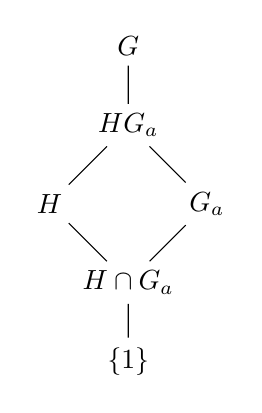
\begin{tikzpicture}
				\node (G) at (0, 0) {$G$};
				\node (HGa) at (0, -1) {$HG_a$};
				\node (H) at (-1, -2) {$H$};
				\node (Ga) at (1, -2) {$G_a$};
				\node (HcapGa) at (0, -3) {$H \cap G_a$};
				\node (1) at (0, -4) {$\{1\}$};

				\draw (1) -- (HcapGa) -- (H) -- (HGa) -- (G);
				\draw (HcapGa) -- (Ga) -- (HGa);
			\end{tikzpicture}
		\end{center}
	\end{solalph}
	\item Let $H$ and $K$ be subgroups of the group $G$. For each $x \in G$ define the $HK$ \textit{double coset} of $x$ in $G$ to be the set $HxK = \{hxk \mid h \in H, k \in K\}$.
	\begin{problems}
		\item Prove that $HxK$ is the union of the left cosets $x_1K, \ldots, x_nK$ where $\{x_1K, \ldots, x_nK\}$ is the orbit containing $xK$ of $H$ acting by left multiplication on the set of left cosets of $K$.
		\item Prove that $HxK$ is a union of right cosets of $H$.
		\item Show that $HxK$ and $HyK$ are either the same set or are disjoint for all $x, y \in G$. Show that the set of $HK$ double cosets partitions $G$.
		\item Prove that $|HxK| = |K| \cdot |H : H \cap xKx^{-1}|$.
		\item Prove that $|HxK| = |H| \cdot |K : K \cap x^{-1}Hx|$.
	\end{problems}
	\begin{solalph}
		\item Let $\oo$ be the orbit containing $xK$ of $H$ acting by left multiplication on the set of left cosets of $K$. Then $\oo = \set{hxK \mid h \in H}$, and let $\{x_1K, \ldots, x_nK\}$ be the distinct left cosets in $\oo$. Let $\kk$ be the union of these left cosets, i.e., $\kk = \bigcup_1^n x_iK$.
		
		Now pick $y \in HxK$. Then there exist $h \in H$ and $k \in K$ such that $y = hxk$. Note that $hxK \in \oo$, so there exists some $i$ such that $hxK = x_iK$. Therefore, $y = hxk \in x_iK \subseteq \kk$, hence $HxK \subseteq \kk$. If $z \in \kk$, then there exists some $i$ and some $k' \in K$ such that $z = x_ik'$. Since $x_iK \in \oo$, then there exists some $h' \in H$ such that $x_iK = h'xK$, hence $x_i = h'xk''$ for some $k'' \in K$. Therefore, $z = x_ik' = h'xkk'' \in HxK$, so $\kk \subseteq HxK$. We have shown that $HxK = \kk$, i.e., $HxK$ is the union of the left cosets $x_1K, \ldots, x_nK$.
		\item The proof is similar to that of part (a). 
		\item Let $x, y \in G$. Suppose $HxK \cap HyK \neq \emptyset$. Then there exist $h_1, h_2 \in H$ and $k_1, k_2 \in K$ such that $h_1 x k_1 = h_2 y k_2$. Rearranging, we have $y = h_2\inv h_1 x k_1 k_2\inv$, hence $y \in HxK$. Therefore, $HyK \subseteq HxK$. By symmetry, we also have $HxK \subseteq HyK$, so $HxK = HyK$. We have shown that $HxK$ and $HyK$ are either the same set or are disjoint for all $x, y \in G$. Since every element of $G$ is in some double coset of the form $HxK$, then the set of $HK$ double cosets partitions $G$.
		\item Recall that the orbit of $xK$ under this action is $\oo = \set{hxK \mid h \in H}$. By Proposition 4.2, we have $|\oo| = |H : H_{xK}|$, where $H_{xK}$ is the stabilizer of $xK$ in $H$. Observe that $H_{xK} = \set{h \in H \mid hxK = xK}$. Then $hxK = xK$ implies that there exists some $k \in K$ such that $hxk = x$, or equivalently, $h = x k x\inv$. Therefore, $H_{xK} = H \cap x K x\inv$. By part (a), we have $|HxK| = |\oo| \cdot |K| = |H : H \cap x K x\inv| \cdot |K|$.
		\item Similar to part (d).
	\end{solalph}
\end{problems}

\newpage

\subsection{Groups Acting on Themselves by Left Mutliplication---Cayley's Theorem}

\begin{problems}
	\item Let $G$ be $\{1,a,b,c\}$, the Klein 4-group whose group table is written out in Section 2.5.
	\begin{problems}
		\item Label $1,a,b,c$ with the integers $1,2,4,3$, respectively, and prove that under the left regular representation of $G$ into $S_4$ the nonidentity elements are mapped as follows:
		\[a \mapsto (1\,2)(3\,4), \quad b \mapsto (1\,4)(2\,3), \quad c \mapsto (1\,3)(2\,4).\]
		\item Relabel $1,a,b,c$ as $1,4,2,3$, respectively, and compute the image of each element of $G$ under the left regular representation of $G$ into $S_4$. Show that the image of $G$ in $S_4$ under this labelling is the same \emph{subgroup} as the image of $G$ in part (a) (even though the nonidentity elements individually map to different permutations under the two different labellings).
	\end{problems}
	\begin{solalph}
		\item We have $a \cdot 1 = a$ so that $\sigma_a(1) = 2$. Similarly, $\sigma_a(2) = 1$. We also have $a \cdot b = c$ so that $\sigma_a(4) = 3$, and $\sigma_a(3) = 4$, and we have $a \mapsto (1\ 2)(3\ 4)$. The others are computed similarly. 
		\item Again, we have $a \cdot 1 = a$ so that $\sigma_a(1) = 4$. Similarly, $\sigma_a(4) = 1$. We also have $a \cdot b = c$ so that $\sigma_a(2) = 3$, and $\sigma_a(3) = 2$, and we have $a \mapsto (1\ 4)(2\ 3)$. For $b$, we have $b \mapsto (1\ 2)(3\ 4)$, and for $c$, we have $c \mapsto (1\ 3)(2\ 4)$. The image of $G$ in $S_4$ under this labelling is $\{1, (1\ 4)(2\ 3), (1\ 2)(3\ 4), (1\ 3)(2\ 4)\}$, which is the same subgroup as in part (a).
	\end{solalph}
	\item List the elements of $S_3$ as $1, (1\,2), (2\,3), (1\,3), (1\,2\,3), (1\,3\,2)$ and label these with the integers $1,2,3,4,5,6$ respectively. Exhibit the image of each element of $S_3$ under the left regular representation of $S_3$ into $S_6$.
	\begin{sol}
		Consider $(1\ 2)$. Then we have the following computations:
		\begin{align*}
			(1\ 2) \cdot 1 & = (1\ 2) && \sigma_{(1\ 2)}(1) = 2 \\
			(1\ 2) \cdot (1\ 2) & = 1 && \sigma_{(1\ 2)}(2) = 1 \\
			(1\ 2) \cdot (2\ 3) & = (1\ 3\ 2) && \sigma_{(1\ 2)}(4) = 5 \\
			(1\ 2) \cdot (1\ 3) & = (1\ 2\ 3) && \sigma_{(1\ 2)}(3) = 6 \\
			(1\ 2) \cdot (1\ 2\ 3) & = (2\ 3) && \sigma_{(1\ 2)}(5) = 3 \\
			(1\ 2) \cdot (1\ 3\ 2) & = (1\ 3) && \sigma_{(1\ 2)}(6) = 4
		\end{align*}
		Thus, we have $(1\ 2) \mapsto (1\ 2)(3\ 6\ 4\ 5)$. We calculate that $(2\ 3) \mapsto (1\ 3\ 5\ 2)(4\ 6)$. Since $(1\ 2)(2\ 3) = (1\ 2\ 3)$, then
		\[(1\ 2\ 3) \mapsto (1\ 2)(3\ 6\ 4\ 5)(1\ 3\ 5\ 2)(4\ 6) = (1\ 5\ 6)(2\ 4\ 3)\]
		Continuing in this way, we find that the images of the elements of $S_3$ under the left regular representation are as follows:
		\begin{align*}
			1 & \mapsto 1 \\
			(1\ 2) & \mapsto (1\ 2)(3\ 6\ 4\ 5) \\
			(2\ 3) & \mapsto (1\ 3\ 5\ 2)(4\ 6) \\
			(1\ 3) & \mapsto (1\ 4)(2\ 6)(3\ 5) \\
			(1\ 2\ 3) & \mapsto (1\ 5\ 6)(2\ 4\ 3) \\
			(1\ 3\ 2) & \mapsto (1\ 6\ 5)(2\ 3\ 4) \qh
		\end{align*}
	\end{sol}
	\item Let $r$ and $s$ be the usual generators for the dihedral group of order 8.
	\begin{problems}
		\item List the elements of $D_8$ as $1, r, r^2, r^3, s, sr, sr^2, sr^3$ and label these with the integers $1,2,\dots,8$ respectively. Exhibit the image of each element of $D_8$ under the left regular representation of $D_8$ into $S_8$.
		\item Relabel this same list of elements of $D_8$ with the integers $1,3,5,7,2,4,6,8$ respectively and recompute the image of each element of $D_8$ under the left regular representation with respect to this new labelling. Show that the two subgroups of $S_8$ obtained in parts (a) and (b) are different.
	\end{problems}
	\begin{solalph}
		\item We calculate $\sigma_r = (1\ 2\ 3\ 4)(5\ 8\ 7\ 6)$ and $\sigma_s = (1\ 5)(2\ 6)(3\ 7)(4\ 8)$. Continuing in this way, we find that the images of the elements of $D_8$ under the left regular representation are as follows:
		\begin{align*}
			1 & \mapsto 1 & s & \mapsto (1\ 5)(2\ 6)(3\ 7)(4\ 8) \\
			r & \mapsto (1\ 2\ 3\ 4)(5\ 8\ 7\ 6) & sr & \mapsto (1\ 6)(2\ 7)(3\ 8)(4\ 5) \\
			r^2 & \mapsto (1\ 3)(2\ 4)(5\ 7)(6\ 8) & sr^2 & \mapsto (1\ 7)(2\ 8)(3\ 5)(4\ 6) \\
			r^3 & \mapsto (1\ 4\ 3\ 2)(5\ 6\ 7\ 8) & sr^3 & \mapsto (1\ 8)(2\ 5)(3\ 6)(4\ 7)
		\end{align*}
		\item The images of $D_8$ under the left regular representation with respect to this new labelling are as follows:
		\begin{align*}
			1 & \mapsto 1 & s & \mapsto (1\ 2)(3\ 4)(5\ 6)(7\ 8) \\
			r & \mapsto (1\ 3\ 5\ 7)(2\ 8\ 6\ 4) & sr & \mapsto (1\ 4)(2\ 7)(3\ 6)(5\ 8) \\
			r^2 & \mapsto (1\ 5)(3\ 7)(2\ 6)(4\ 8) & sr^2 & \mapsto (1\ 6)(2\ 5)(3\ 8)(4\ 7) \\
			r^3 & \mapsto (1\ 7\ 5\ 3)(2\ 4\ 6\ 8) & sr^3 & \mapsto (1\ 8)(2\ 3)(4\ 5)(6\ 7)
		\end{align*}
		Clearly, the two subgroups of $S_8$ obtained in parts (a) and (b) are different since, for example, the image of $r$ in part (a) is a product of two 4-cycles while the image of $r$ in part (b) is a product of two 4-cycles but with different elements.
	\end{solalph}
	\item \label{ex4.2.4} Use the left regular representation of $Q_8$ to produce two elements of $S_8$ which generate a subgroup of $S_8$ isomorphic to the quaternion group $Q_8$.
	\begin{sol}
		At minimum, we have that $Q_8 = \gen{i, j}$ (any 2 elements of order 4 can be used), so we compute the images of $i$ and $j$ under the left regular representation. We label $Q_8$ as $1, -1, i, -i, j, -j, k, -k$ and label these with the integers $1,2 \ldots 8$ respectively. We find that
		\begin{align*}
			i & \mapsto \sigma_i = (1\ 3\ 4\ 2)(5\ 7)(6\ 8) \\
			j & \mapsto \sigma_j = (1\ 5\ 2\ 6)(3\ 8)(4\ 7)
		\end{align*}
		Hence $Q_8 \cong \gen{\sigma_i, \sigma_j} \leq S_8$.
	\end{sol}
	\item Let $r$ and $s$ be the usual generators for the dihedral group of order 8 and let $H = \langle s \rangle$. List the left cosets of $H$ in $D_8$ as $1H, rH, r^2H$ and $r^3H$.
	\begin{problems}
		\item Label these cosets with the integers $1,2,3,4$, respectively. Exhibit the image of each element of $D_8$ under the representation $\pi_H$ of $D_8$ into $S_4$ obtained from the action of $D_8$ by left multiplication on the set of 4 left cosets of $H$ in $D_8$. Deduce that this representation is faithful (i.e., the elements of $S_4$ obtained form a subgroup isomorphic to $D_8$).
		\item Repeat part (a) with the list of cosets relabelled by the integers $1,3,2,4$, respectively. Show that the permutations obtained from this labelling form a subgroup of $S_4$ that is different from the subgroup obtained in part (a).
		\item Let $K = \langle sr \rangle$, list the cosets of $K$ in $D_8$ as $1K, rK, r^2K$ and $r^3K$, and label these with the integers $1,2,3,4$. Prove that, with respect to this labelling, the image of $D_8$ under the representation $\pi_K$ obtained from left multiplication on the cosets of $K$ is the same \emph{subgroup} of $S_4$ as in part (a) (even though the subgroups $H$ and $K$ are different and some of the elements of $D_8$ map to different permutations under the two homomorphisms).
	\end{problems}
	\begin{solalph}
		\item We have $\pi_H(r) = (1\ 2\ 3\ 4)$ and $\pi_H(s) = (2\ 4)$. We continue in this way to find that the images of the elements of $D_8$ under $\pi_H$ are:
		\begin{align*}
			\pi_H(1) & = 1 & \pi_H(s) & = (2\ 4) \\
			\pi_H(r) & = (1\ 2\ 3\ 4) & \pi_H(sr) & = (1\ 2)(3\ 4) \\
			\pi_H(r^2) & = (1\ 3)(2\ 4) & \pi_H(sr^2) & = (1\ 3) \\
			\pi_H(r^3) & = (1\ 4\ 3\ 2) & \pi_H(sr^3) & = (1\ 4)(2\ 3)
		\end{align*}
		so that the subgroup $\gen{\pi_H(r), \pi_H(s)} \leq S_4$ is isomorphic to $D_8$. Since the kernel of $\pi_H$ is trivial, then the representation is faithful.
		\item The new labelling affords the permutations $\pi_H(r) = (1\ 3\ 2\ 4)$ and $\pi_H(s) = (3\ 4)$. We have the following images:
		\begin{align*}
			\pi_H(1) & = 1 & \pi_H(s) & = (3\ 4) \\
			\pi_H(r) & = (1\ 3\ 2\ 4) & \pi_H(sr) & = (1\ 3)(2\ 4) \\
			\pi_H(r^2) & = (1\ 2)(3\ 4) & \pi_H(sr^2) & = (1\ 2) \\
			\pi_H(r^3) & = (1\ 4\ 2\ 3) & \pi_H(sr^3) & = (1\ 4)(2\ 3)
		\end{align*}
		Moreover, the subgroup is different from that in part (a) since, for example, the image of $r$ in part (a) is $(1\ 2\ 3\ 4)$ while the image of $r$ in this part is $(1\ 3\ 2\ 4)$.
		\item Under $\pi_K$, we have $\pi_K(r) = (1\ 2\ 3\ 4)$ and $\pi_K(s) = (1\ 2)(3\ 4)$. With respect to this labeling, we have the subgroup $\wh K = \gen{(1\ 2\ 3\ 4), (1\ 2)(3\ 4)}$. Let $\wh H$ be the subgroup obtained in part (a). Note that $(1\ 2\ 3\ 4)$ is contained in both $\wh H$ and $\wh K$. Moreover, we have following:
		\[(1\ 2\ 3\ 4)(2\ 4)(1\ 4\ 3\ 2) = (1\ 2)(3\ 4) \in \wh H \longand (1\ 2\ 3\ 4)^2(1\ 2)(3\ 4) = (2\ 4) \in \wh K\]
		so that both subgroups contain the other generator of the other subgroup. Therefore, $\wh H = \wh K$.
	\end{solalph}
    \item Let $r$ and $s$ be the usual generators for the dihedral group of order 8 and let $N = \langle r^2 \rangle$. List the left cosets of $N$ in $D_8$ as $1N, rN, sN$ and $srN$. Label these cosets with the integers $1,2,3,4$ respectively. Exhibit the image of each element of $D_8$ under the representation $\pi_N$ of $D_8$ into $S_4$ obtained from the action of $D_8$ by left multiplication on the set of 4 left cosets of $N$ in $D_8$. Deduce that this representation is not faithful and prove that $\pi_N(D_8)$ is isomorphic to the Klein 4-group.
	\begin{sol}
		We have $\pi_N(r) = (1\ 2)(3\ 4)$ and $\pi_N(s) = (1\ 3)(2\ 4)$. Continuing in this way, we find that the images of the elements of $D_8$ under $\pi_N$ are:
		\begin{align*}
			\pi_N(1) & = 1 & \pi_N(s) & = (1\ 3)(2\ 4) \\
			\pi_N(r) & = (1\ 2)(3\ 4) & \pi_N(sr) & = (1\ 4)(2\ 3) \\
			\pi_N(r^2) & = 1 & \pi_N(sr^2) & = (1\ 3)(2\ 4) \\
			\pi_N(r^3) & = (1\ 2)(3\ 4) & \pi_N(sr^3) & = (1\ 4)(2\ 3)
		\end{align*}
		Since $\ker(\pi_N)$ contains the nontrivial element $r^2$, then the representation is not faithful. Moreover, we have $\pi_N(D_8) = \{1, (1\ 2)(3\ 4), (1\ 3)(2\ 4), (1\ 4)(2\ 3)\}$, which is isomorphic to the Klein 4-group.
	\end{sol}
    \item Let $Q_8$ be the quaternion group of order 8.
	\begin{problems}
		\item Prove that $Q_8$ is isomorphic to a subgroup of $S_8$.
		\item Prove that $Q_8$ is not isomorphic to a subgroup of $S_n$ for any $n \le 7$. [If $Q_8$ acts on any set $A$ of order $\le 7$ show that the stabilizer of any point $a \in A$ must contain the subgroup $\langle -1 \rangle$.]
	\end{problems}
	\begin{solalph}
		\item This is done in \hyperref[ex4.2.4]{Exercise 4.2.4}.
		\item Let $Q_8$ act on a set $A$ of order $n \leq 7$. For any $a \in A$, consider the orbit $\oo_a$ of $a$ under this action. By Proposition 4.2, we have $|\oo_a| = |Q_8 : (Q_8)_a|$, where $(Q_8)_a$ is the stabilizer of $a$ in $Q_8$. Since $|\oo_a|$ divides $|A| \leq 7$, then $|\oo_a|$ must be 1, 2, 4, or 7. However, since $Q_8$ has no subgroup of index 7, then $|\oo_a|$ cannot be 7. If $|\oo_a| = 4$, then $(Q_8)_a$ has order 2, but the only subgroup of order 2 in $Q_8$ is $\langle -1 \rangle$. If $|\oo_a| = 2$, then $(Q_8)_a$ has order 4, and the only subgroups of order 4 in $Q_8$ are $\langle i \rangle$, $\langle j \rangle$, and $\langle k \rangle$, all of which contain $\langle -1 \rangle$. If $|\oo_a| = 1$, then $(Q_8)_a = Q_8$, which also contains $\langle -1 \rangle$. Therefore, in all cases, the stabilizer $(Q_8)_a$ contains $\langle -1 \rangle$. Since this holds for all $a \in A$, then $\langle -1 \rangle$ is contained in the kernel of the action. The action is not faithful, hence $Q_8$ cannot be isomorphic to a subgroup of $S_n$ for any $n \leq 7$.
	\end{solalph}
    \item Prove that if $H$ has finite index $n$ then there is a normal subgroup $K$ of $G$ with $K \le H$ and $|G : K| \le n!$.
	\begin{sol}
		Let $G$ act by left multiplication on the set of left cosets of $H$ in $G$. Then we have the homomorphism $\phi : G \to S_n$, which is the permutation representation of $G$ on $G/H$. Let $K = \ker(\phi) \subseteq H$, since $g \in K$ if and only if $gH = H$. By the First Isomorphism Theorem, we have $G/K \cong \phi(G) \leq S_n$, so that $|G : K| = |G/K| = |\phi(G)|$ divides $n!$. Therefore, $|G : K| \leq n!$.
	\end{sol}
    \item Prove that if $p$ is a prime and $G$ is a group of order $p^\alpha$ for some $\alpha \in \mathbb{Z}^+$, then every subgroup of index $p$ is normal in $G$. Deduce that every group of order $p^2$ has a normal subgroup of order $p$.
	\begin{sol}
		Let $H$ be a subgroup of $G$ with index $p$. Then $|G : H| = p$, so the action of $G$ on the left cosets of $H$ in $G$ gives a homomorphism $\phi : G \to S_p$. Since $|G| = p^\alpha$, then by Lagrange's Theorem, the order of $\phi(G)$ divides $p^\alpha$. However, the only subgroups of $S_p$ whose order divides $p^\alpha$ are the trivial group and groups of order $p$. Since $\phi(G)$ acts transitively on the $p$ cosets of $H$, then $\phi(G)$ cannot be trivial. Therefore, $|\phi(G)| = p$, which is prime, so $\phi(G)$ is cyclic and hence abelian. The kernel of $\phi$ is a normal subgroup of $G$ contained in $H$. Since the image $\phi(G)$ has order $p$, then by the First Isomorphism Theorem, we have $|G : \ker(\phi)| = p$. But since $\ker(\phi) \subseteq H$ and both have index $p$, then $\ker(\phi) = H$. Therefore, $H$ is normal in $G$.

		To deduce that every group of order $p^2$ has a normal subgroup of order $p$, let $G$ be a group of order $p^2$. By Cauchy's Theorem, there exists an element of order $p$ in $G$, which generates a subgroup $H$ of order $p$. Since the index of $H$ in $G$ is $p$, by the previous result, $H$ is normal in $G$.
	\end{sol}
    \item Prove that every non-abelian group of order 6 has a nonnormal subgroup of order 2. Use this to classify groups of order 6. [Produce an injective homomorphism into $S_3$.]
	\begin{sol}
		Note that $2 \mid 6$ and $3 \mid 6$. By Cauchy's Theorem, there exists subgroups $H$ and $K$ of orders 2 and 3 respectively. Let $H = \set{1, h}$, suppose it is normal, and let $g \in G - H$. Since $H \nsub G$, then $gHg\inv = H$. In particular, $ghg\inv \in H$, so either $ghg\inv = 1$ or $ghg\inv = h$. Since the first case implies $h = 1$, it must be that $ghg\inv = h$, or $gh = hg$. Then $h$ commutes with every element. Moreover, we may use \hyperref[ex3.3.3]{Exercise 3.3.3} to conclude that $G = HK$ since $H \nsub G$. Since $K$ is also abelian as it is cyclic, then $G = hk$ for $h \in H$ and $k \in K$, implying that $G$ is abelian, a contradiction. Therefore, $H$ is not normal in $G$.

		To classify groups of order 6, let $G$ be a group of order 6. If $G$ is abelian, then $G \cong \z_6 \cong \z_2 \times \z_3$. If $G$ is non-abelian, then by the above result, $G$ has a nonnormal subgroup $H$ of order 2. Let $K$ be the subgroup of order 3. Then $G = HK$. Let $G$ act by left multiplication on the left cosets of $K$ in $G$. This action gives a homomorphism $\phi : G \to S_3$. Since $H$ is not normal in $G$, then the action is nontrivial, so $\phi$ is injective. Therefore, $G \cong \phi(G) \leq S_3$. Since $|G| = 6 = |S_3|$, then $\phi(G) = S_3$, and hence $G \cong S_3$.
	\end{sol}
    \item \label{ex4.2.11} Let $G$ be a finite group and let $\pi : G \to S_G$ be the left regular representation. Prove that if $x$ is an element of $G$ of order $n$ and $|G| = mn$, then $\pi(x)$ is a product of $m$ $n$-cycles. Deduce that $\pi(x)$ is an odd permutation if and only if $|x|$ is even and $\abs G/\abs x$ is odd.
	\begin{sol}
		Let $x \in G$ with $\abs x = n$. Consider the action of $\langle x \rangle$ on $G$ by left multiplication. The orbit of any $g \in G$ under this action is $\oo_g = \set{x^k g \mid k = 0, 1, \ldots, n-1}$. Since $\abs x = n$, then $|\oo_g| = n$ for all $g \in G$. By Proposition 4.2, we have $|\oo_g| = |\langle x \rangle : (\langle x \rangle)_g|$, where $(\langle x \rangle)_g$ is the stabilizer of $g$ in $\langle x \rangle$. Since $|\oo_g| = n$, then $(\langle x \rangle)_g$ is trivial for all $g \in G$. Therefore, the orbits of this action partition $G$ into subsets of size $n$. Since $|G| = mn$, there are exactly $m$ such orbits. Each orbit corresponds to an $n$-cycle in the permutation $\pi(x)$. Therefore, $\pi(x)$ is a product of $m$ $n$-cycles.

		To determine when $\pi(x)$ is an odd permutation, we note that an $n$-cycle is an odd permutation if and only if $n$ is even. Since $\pi(x)$ is a product of $m$ $n$-cycles, the parity of $\pi(x)$ is determined by the parity of $m$ and $n$. Specifically, $\pi(x)$ is odd if and only if $n$ is even and $m$ is odd. Thus, $\pi(x)$ is an odd permutation if and only if $|x|$ is even and $|G|/|x|$ is odd.
	\end{sol}
    \item \label{ex4.2.12} Let $G$ and $\pi$ be as in the preceding exercise. Prove that if $\pi(G)$ contains an odd permutation then $G$ has a subgroup of index 2. [Use \hyperref[ex3.3.3]{Exercise 3.3.3}.]
	\begin{sol}
		Recall the $\ep$ homomorphism from Proposition 3.23. Moreover, $\pi$ is a homomorphism from $G$ to $S_G$. Consider the composition $\ep \circ \pi : G \to \set{\pm 1}$. Since $\pi(G)$ contains an odd permutation, then $\ep \circ \pi$ is surjective. By the First Isomorphism Theorem, we have $G/\ker(\ep \circ \pi) \cong \set{\pm 1}$, so that $|\ker(\ep \circ \pi)| = |G|/2$. Therefore, $\ker(\ep \circ \pi)$ is a subgroup of $G$ of index 2.
	\end{sol}
    \item Prove that if $|G| = 2k$ where $k$ is odd then $G$ has a subgroup of index 2. [Use Cauchy's Theorem to produce an element of order 2 and then use the preceding two exercises.]
	\begin{sol}
		By Cauchy's Theorem, there exists $x \in G$ such that $\abs x = 2$. Then $\pi(x)$ is of order 2 and is hence a product of disjoint transpositions. Since $|G| = 2k$ with $k$ odd, then use $m = k$ and $n = 2$ in \hyperref[ex4.2.11]{Exercise 4.2.11} along with even $\abs x$ to conclude that $\pi(x)$ is an odd permutation. By the \hyperref[ex4.2.12]{Exercise 4.2.12}, $G$ has a subgroup of index 2.
	\end{sol}
    \item Let $G$ be a finite group of composite order $n$ with the property that $G$ has a subgroup of order $k$ for each positive integer $k$ dividing $n$. Prove that $G$ is not simple.
    \begin{sol}
		Let $S$ be the set of all prime factors of $n$. By the Well Ordering Principle, this has a minimal element $p$. By hypothesis, $G$ has a subgroup $P$ of order $n/p$ with index $p$. By Corollary 4.5, $P$ is normal in $G$ since $p$ is the smallest prime dividing $n$. Therefore, $G$ is not simple.
	\end{sol}
\end{problems}
